% Modern editorial, markup and figure/layout contributions: CC-BY-SA-4.0.
% Historical text and illustrations: Leonhard Euler (1744), public domain.
% Component scope and upstream attribution: see RIGHTS.md.
% Manual vector redrawing after E65, Tabula IV. Schematic coordinates; original point relations retained.
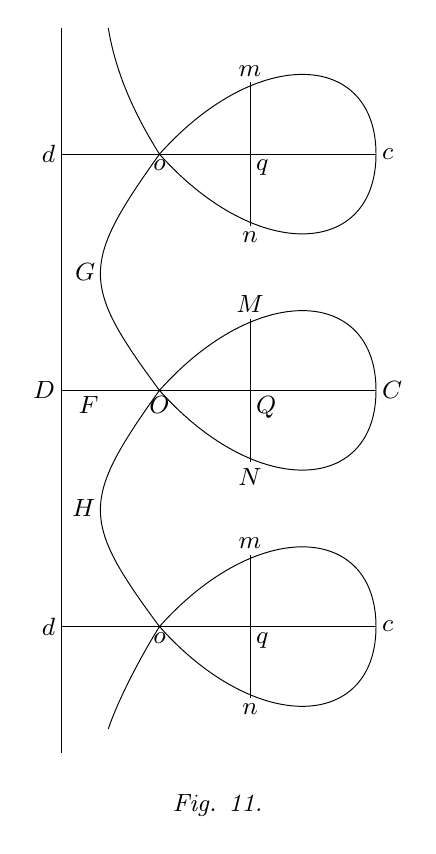
\begin{tikzpicture}[x=1cm,y=1cm,line width=.35pt,font=\small]
\draw (0,-4.6)--(0,4.6);
\draw (.6,4.6)..controls (.7,4) and (.95,3.48)..(1.25,3)..controls (2.5,1.6) and (4,1.7)..(4,3)..controls (4,4.3) and (2.5,4.4)..(1.25,3)..controls (.25,1.6) and (.25,1.35)..(1.25,0)..controls (2.5,-1.4) and (4,-1.3)..(4,0)..controls (4,1.3) and (2.5,1.4)..(1.25,0)..controls (.25,-1.4) and (.25,-1.65)..(1.25,-3)..controls (2.5,-4.4) and (4,-4.3)..(4,-3)..controls (4,-1.7) and (2.5,-1.6)..(1.25,-3)..controls (.95,-3.48) and (.7,-4)..(.6,-4.3);
\foreach \y in {-3,0,3}{\draw (0,\y)--(4,\y) (2.4,{\y-.91})--(2.4,{\y+.91});}
\node[left,inner sep=2pt] at (0,3) {$d$};
\node[below,inner sep=2pt] at (1.25,3) {$o$};
\node[right,inner sep=2pt] at (4,3) {$c$};
\node[above,inner sep=2pt] at (2.4,3.91) {$m$};
\node[below,inner sep=2pt] at (2.4,2.09) {$n$};
\node[below right,inner sep=2pt] at (2.4,3) {$q$};
\node[left,inner sep=2pt] at (0,0) {$D$};
\node[below,inner sep=2pt] at (0.35,0) {$F$};
\node[below,inner sep=2pt] at (1.25,0) {$O$};
\node[right,inner sep=2pt] at (4,0) {$C$};
\node[above,inner sep=2pt] at (2.4,0.91) {$M$};
\node[below,inner sep=2pt] at (2.4,-0.91) {$N$};
\node[below right,inner sep=2pt] at (2.4,0) {$Q$};
\node[left,inner sep=2pt] at (0.51,1.5) {$G$};
\node[left,inner sep=2pt] at (0.51,-1.5) {$H$};
\node[left,inner sep=2pt] at (0,-3) {$d$};
\node[below,inner sep=2pt] at (1.25,-3) {$o$};
\node[right,inner sep=2pt] at (4,-3) {$c$};
\node[above,inner sep=2pt] at (2.4,-2.09) {$m$};
\node[below,inner sep=2pt] at (2.4,-3.91) {$n$};
\node[below right,inner sep=2pt] at (2.4,-3) {$q$};
\node[anchor=north] at ([yshift=-4mm]current bounding box.south) {\textit{Fig. 11.}};
\end{tikzpicture}
